\chapter{Implementation Details}

\subsection{Network Discovery}
\begin{SCfigure}
    \centering
    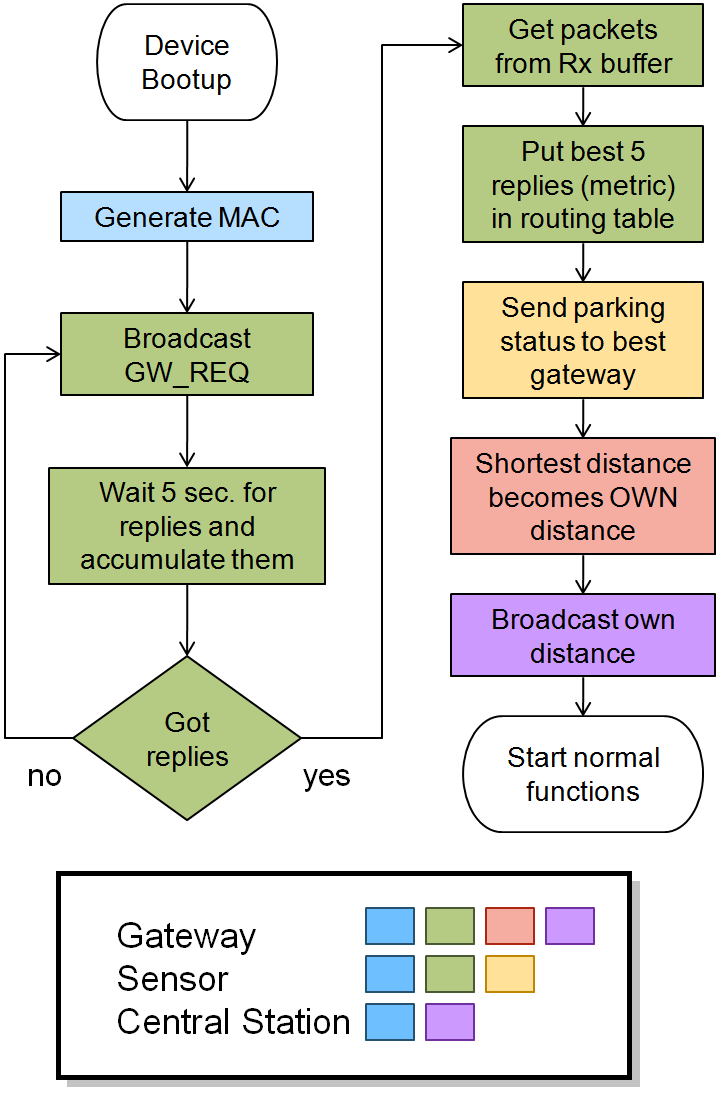
\includegraphics[width=8cm]{images/Flowchart_NetworkDiscovery.png}
	\vspace{-1.5em}
    \caption{Network discovery process for the three roles.}
    \vspace{-1.5em}
    \label{fig:network_discovery}
\end{SCfigure}

\subsection{Parking Status Propagation}
\begin{figure}
    \centering
    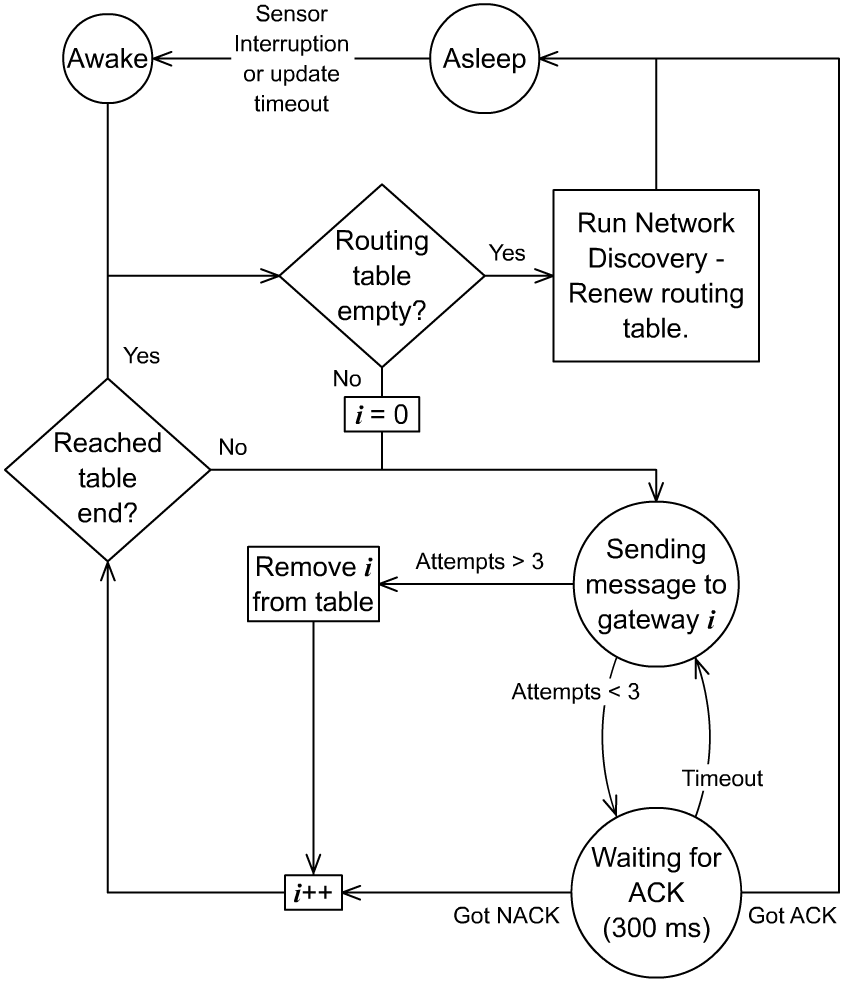
\includegraphics[width=10cm]{images/Flowchart_Mote.png}
	\vspace{-1.5em}
    \caption{Flowchart of the functions of a sensor.}
    \vspace{-1.5em}
    \label{fig:sensor}
\end{figure}

\begin{figure}
    \centering
    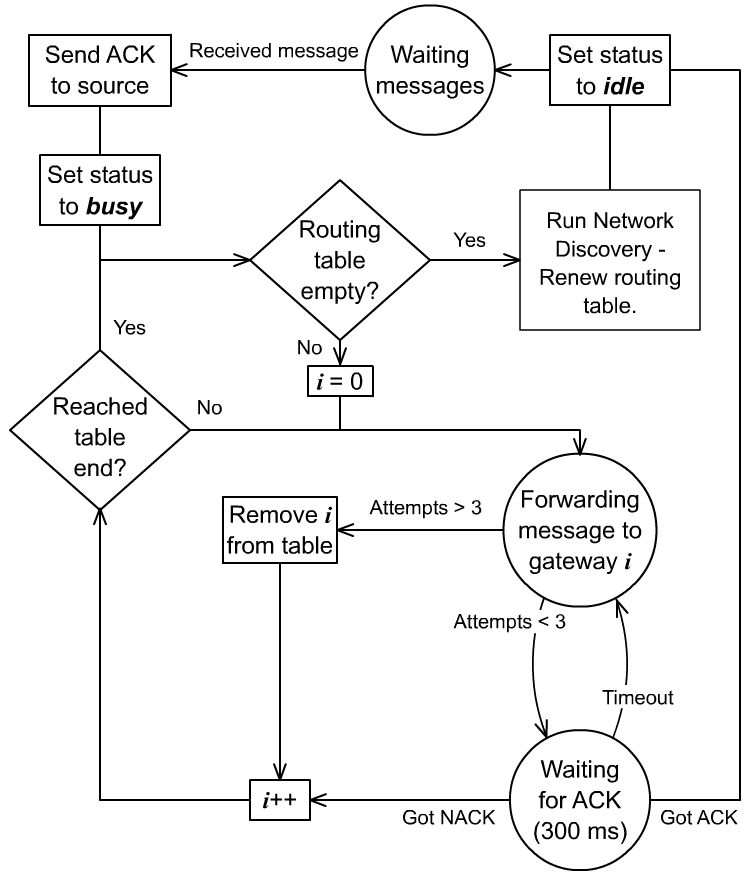
\includegraphics[width=10cm]{images/Flowchart_Gateway.png}
	\vspace{-1.5em}
    \caption{Flowchart of the functions of a gateway.}
    \vspace{-1.5em}
    \label{fig:gateway}
\end{figure}

\subsection{Packet Format}
\begin{figure}
    \centering
    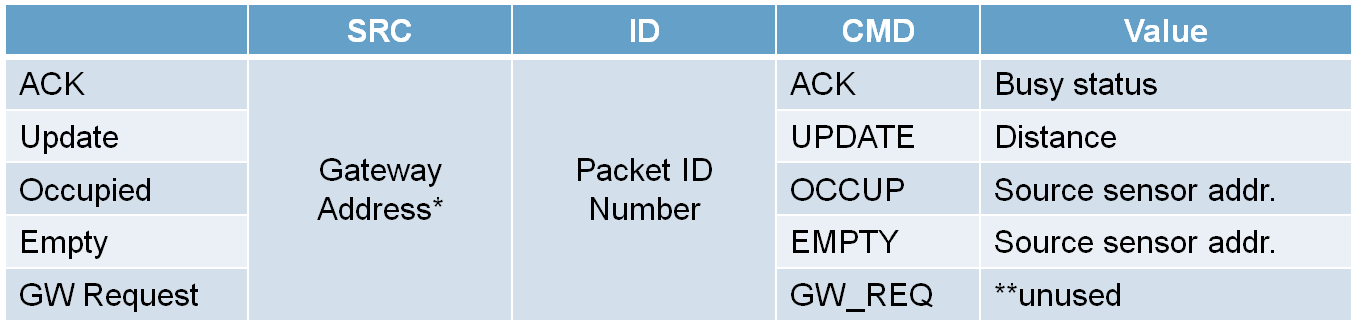
\includegraphics[width=15cm]{images/General_PacketFormat.png}
	\vspace{-1.5em}
    \caption[Packet format]{Packet Format. 
	\(\ast\) In the case of occupied and empty, the SRC field originally contains the sensor's address.
	\(\ast\ast\) The Packet is fixed length, so the unused value is arbitrarily assigned.}
    \vspace{-1.5em}
    \label{fig:packet}
\end{figure}

\subsection{Hardware used}

\subsection{Graphical User Interface}

